%==============================================================================%
%                                DOCUMENT CLASS                                %
%==============================================================================%
\documentclass[11pt]{standalone}

%==============================================================================%
%                                   PACKAGES                                   %
%==============================================================================%
% A better bold face
\usepackage{bm}

% Cool colours
\usepackage{color}
\usepackage[usenames, dvipsnames]{xcolor}

% tikz - for drawing stuff
\usepackage{tikz}

%==============================================================================%
%                                PACKAGE SETUP                                 %
%==============================================================================%
% Boxes around stuff
\usetikzlibrary{fit,calc}
\usetikzlibrary{shapes.geometric, arrows, chains}

\tikzset{
  minimum width = 4.6cm,
  minimum height = 0.8cm,
  %---------------------------------------%
  %  Single-Filter: Two-Level Atom boxes  %
  %---------------------------------------%
  % Box for the Atomic Moments
  box_auto_sigma/.style={
    rectangle,
    rounded corners,
    align=center,
    draw=black,
    fill=red!30
  },
  % Box for the first-order filter moments
  box_auto_f1/.style={
    rectangle,
    rounded corners,
    align=center,
    draw=black,
    fill=yellow!30
  },
  % Box for the second-order filter moments
  box_auto_f2/.style={
    rectangle,
    rounded corners,
    align=center,
    draw=black,
    fill=green!30
  },
  % Box for the third-order filter moments
  box_auto_f3/.style={
    rectangle,
    rounded corners,
    align=center,
    draw=black,
    fill=cyan!30
  },
  % Box for the fourth-order filter moments
  box_auto_f4/.style={
    rectangle,
    rounded corners,
    align=center,
    draw=black,
    fill=magenta!30
  },
  %----------------%
  %     Arrows     %
  %----------------%
  arrow/.style={draw,thick,->,>=stealth},
  dec/.style={
    ellipse,
    align=center,
    draw=black,
    fill=green!30
  },
}

%==============================================================================%
%                               DEFINING COMMANDS                              %
%==============================================================================%
%----------------------------------%
%     COMMANDS TO CHANGE STYLE     %
%----------------------------------%
% Define \op command as a replacement for the \hat{} command. If I change my mind
% later on in writing and don't want the hats, I can just change the definition.
\newcommand{\op}[1]{%
  % Keep that hats
  % {}\hat{#1}
  % Don't keep the hats
  {#1}
}

%==============================================================================%
%                                BEGIN DOCUMENT                                %
%==============================================================================%
%\begin{document}
%  \begin{tikzpicture}[node distance=0.4cm, every edge/.style={arrow}]
%    %------------------%
%    %  Atomic Moments  %
%    %------------------%
%    % Atom
%    \node (sigma) [box_auto_sigma] at (0, 0) {\scalebox{1.0}{$ \langle \op{\bm{\sigma}} \rangle $}};
%
%    %-----------------------%
%    %  First-Order: Filter  %
%    %-----------------------%
%    % First-order: Filter
%    \node (f1) [box_auto_f1] at (4.0, -1.5)  {\scalebox{1.0}{$ \langle \op{a_{j}} \rangle ,  \langle \op{a}^{\dagger}_{j} \rangle $}};
%    % First-order: Filter / Atom
%    \node (f1_sigma) [box_auto_f1] at (0, -1.5)  {\scalebox{1.0}{$ \langle \op{a}_{j} \op{\bm{\sigma}} \rangle ,  \langle \op{a}^{\dagger}_{j} \op{\bm{\sigma}} \rangle $}};
%
%    %--------=---------------%
%    %  Second-Order: Filter  %
%    %------------------------%
%    % Second-order: Filter
%    \node (f2) [box_auto_f2] at (5, -2.25) {\scalebox{1.0}{$ \langle \op{a}_{j} \op{a}_{k} \rangle , \langle \op{a}^{\dagger}_{j} \op{a}^{\dagger}_{k} \rangle,  \langle \op{a}^{\dagger}_{j} \op{a}_{k} \rangle $}};
%    % Second-order: Filter / Atom
%    \node (f2_sigma) [box_auto_f2] at (0, -3.0) {\scalebox{1.0}{$ \langle \op{a}_{j} \op{a}_{k} \op{\bm{\sigma}} \rangle , \langle \op{a}^{\dagger}_{j} \op{a}^{\dagger}_{k} \op{\bm{\sigma}} \rangle , \langle  \op{a}^{\dagger}_{j} \op{a}_{k} \op{\bm{\sigma}} \rangle $}};
%
%    %-------=---------------%
%    %  Third-Order: Filter  %
%    %-----------------------%
%    % Third-order: Filter
%    \node (f3) [box_auto_f3] at (5, -3.75) {\scalebox{1.0}{$ \langle \op{a}^{\dagger}_{j} \op{a}_{k} \op{a}_{l} \rangle , \langle \op{a}^{\dagger}_{j} \op{a}^{\dagger}_{k} \op{a}_{l} \rangle $}};
%    % Third-order: Filter / Atom
%    \node (f3_sigma) [box_auto_f3] at (0, -4.5) {\scalebox{1.0}{$ \langle \op{a}^{\dagger}_{j} \op{a}_{k} \op{a}_{l} \op{\bm{\sigma}} \rangle , \langle \op{a}^{\dagger}_{j} \op{a}^{\dagger}_{k} \op{a}_{k} \op{\bm{\sigma}}  \rangle $}};
%
%    %--------=---------------%
%    %  Fourth-Order: Filter  %
%    %------------------------%
%    % Fourth-order: Filter
%    \node (f4) [box_auto_f4] at (5, -5.25) {\scalebox{1.0}{$ \langle \op{a}^{\dagger}_{j} \op{a}^{\dagger}_{k} \op{a}_{l} \op{a}_{m} \rangle $}};
%
%    %----------%
%    %  Arrows  %
%    %----------%
%    % First-order: Atom --> First-order: Filter
%    \draw [arrow] (sigma.south east) -- (f1.north);
%    % First-order: Atom --> First-order: Filter / Atom
%    \draw [arrow] (sigma.south) -- (f1_sigma.north);
%
%    % First-order: Filter --> First-order: Filter / Atom
%    \draw [arrow] (f1.south) -- (f1_sigma.east);
%    % First-order: Filter / Atom --> Second-order: Filter
%    \draw [arrow] (f1_sigma.east) -- (f2.north);
%    % First-order: Filter / Atom --> Second-order: Filter / Atom
%    \draw [arrow] (f1_sigma.south) -- (f2_sigma.north);
%
%    % Second-order: Filter --> Second-order: Filter / Atom
%    \draw [arrow] (f2) -- (f2_sigma);
%    % Second-order: Filter / Atom --> Third-order: Filter
%    \draw [arrow] (f2_sigma) -- (f3);
%    % Second-order: Filter / Atom --> Third-order: Filter / Atom
%    \draw [arrow] (f2_sigma) -- (f3_sigma);
%
%    % Third-order: Filter --> Third-order: Filter / Atom
%    \draw [arrow] (f3) -- (f3_sigma);
%    % Third-order: Filter / Atom --> Fourth-order: Filter
%    \draw [arrow] (f3_sigma) -- (f4);
%  \end{tikzpicture}
%\end{document}

\begin{document}
  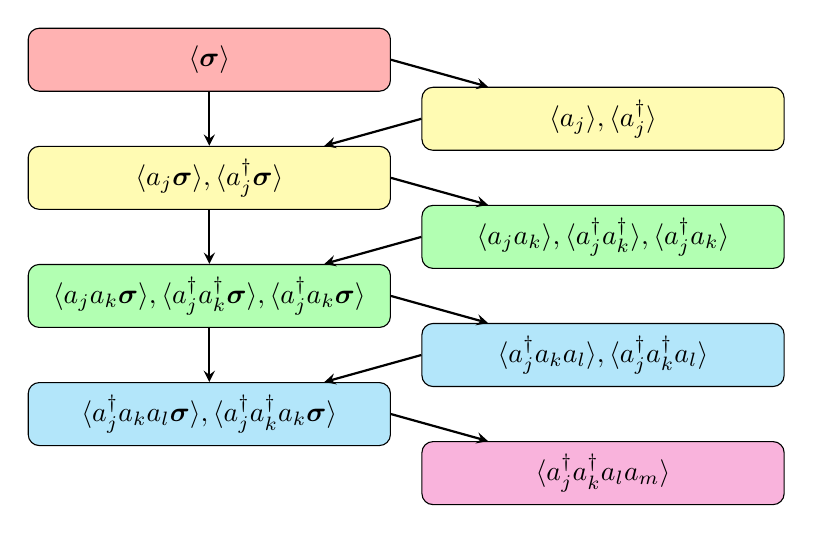
\begin{tikzpicture}[node distance=0.4cm, every edge/.style={arrow}]
    %------------------%
    %  Atomic Moments  %
    %------------------%
    % Atom
    \node (sigma) [box_auto_sigma] at (0, 0) {\scalebox{1.0}{$ \langle \op{\bm{\sigma}} \rangle $}};

    %-----------------------%
    %  First-Order: Filter  %
    %-----------------------%
    % First-order: Filter
    \node (f1) [box_auto_f1] at (5, -0.75)  {\scalebox{1.0}{$ \langle \op{a_{j}} \rangle ,  \langle \op{a}^{\dagger}_{j} \rangle $}};
    % First-order: Filter / Atom
    \node (f1_sigma) [box_auto_f1] at (0, -1.5)  {\scalebox{1.0}{$ \langle \op{a}_{j} \op{\bm{\sigma}} \rangle ,  \langle \op{a}^{\dagger}_{j} \op{\bm{\sigma}} \rangle $}};

    %--------=---------------%
    %  Second-Order: Filter  %
    %------------------------%
    % Second-order: Filter
    \node (f2) [box_auto_f2] at (5, -2.25) {\scalebox{1.0}{$ \langle \op{a}_{j} \op{a}_{k} \rangle , \langle \op{a}^{\dagger}_{j} \op{a}^{\dagger}_{k} \rangle,  \langle \op{a}^{\dagger}_{j} \op{a}_{k} \rangle $}};
    % Second-order: Filter / Atom
    \node (f2_sigma) [box_auto_f2] at (0, -3.0) {\scalebox{1.0}{$ \langle \op{a}_{j} \op{a}_{k} \op{\bm{\sigma}} \rangle , \langle \op{a}^{\dagger}_{j} \op{a}^{\dagger}_{k} \op{\bm{\sigma}} \rangle , \langle  \op{a}^{\dagger}_{j} \op{a}_{k} \op{\bm{\sigma}} \rangle $}};

    %-------=---------------%
    %  Third-Order: Filter  %
    %-----------------------%
    % Third-order: Filter
    \node (f3) [box_auto_f3] at (5, -3.75) {\scalebox{1.0}{$ \langle \op{a}^{\dagger}_{j} \op{a}_{k} \op{a}_{l} \rangle , \langle \op{a}^{\dagger}_{j} \op{a}^{\dagger}_{k} \op{a}_{l} \rangle $}};
    % Third-order: Filter / Atom
    \node (f3_sigma) [box_auto_f3] at (0, -4.5) {\scalebox{1.0}{$ \langle \op{a}^{\dagger}_{j} \op{a}_{k} \op{a}_{l} \op{\bm{\sigma}} \rangle , \langle \op{a}^{\dagger}_{j} \op{a}^{\dagger}_{k} \op{a}_{k} \op{\bm{\sigma}}  \rangle $}};

    %--------=---------------%
    %  Fourth-Order: Filter  %
    %------------------------%
    % Fourth-order: Filter
    \node (f4) [box_auto_f4] at (5, -5.25) {\scalebox{1.0}{$ \langle \op{a}^{\dagger}_{j} \op{a}^{\dagger}_{k} \op{a}_{l} \op{a}_{m} \rangle $}};

    %----------%
    %  Arrows  %
    %----------%
    % First-order: Atom --> First-order: Filter
    \draw [arrow] (sigma.east) -- (f1);
    % First-order: Atom --> First-order: Filter / Atom
    \draw [arrow] (sigma.south) -- (f1_sigma.north);

    % First-order: Filter --> First-order: Filter / Atom
    \draw [arrow] (f1.west) -- (f1_sigma);
    % First-order: Filter / Atom --> Second-order: Filter
    \draw [arrow] (f1_sigma.east) -- (f2);
    % First-order: Filter / Atom --> Second-order: Filter / Atom
    \draw [arrow] (f1_sigma.south) -- (f2_sigma.north);

    % Second-order: Filter --> Second-order: Filter / Atom
    \draw [arrow] (f2.west) -- (f2_sigma);
    % Second-order: Filter / Atom --> Third-order: Filter
    \draw [arrow] (f2_sigma.east) -- (f3);
    % Second-order: Filter / Atom --> Third-order: Filter / Atom
    \draw [arrow] (f2_sigma.south) -- (f3_sigma.north);

    % Third-order: Filter --> Third-order: Filter / Atom
    \draw [arrow] (f3.west) -- (f3_sigma);
    % Third-order: Filter / Atom --> Fourth-order: Filter
    \draw [arrow] (f3_sigma.east) -- (f4);
  \end{tikzpicture}
\end{document}

%\begin{document}
%  \begin{tikzpicture}[node distance=0.4cm, every edge/.style={arrow}]
%    %------------------%
%    %  Atomic Moments  %
%    %------------------%
%    % Atom
%    \node (sigma) [box_auto_sigma] {\scalebox{1.0}{$ \langle \op{\bm{\sigma}} \rangle $}};
%
%    %-----------------------%
%    %  First-Order: Filter  %
%    %-----------------------%
%    % First-order: Filter
%    \node (f1) [box_auto_f1, right=of sigma] {\scalebox{1.0}{$ \langle \op{a_{j}} \rangle ,  \langle \op{a}^{\dagger}_{j} \rangle $}};
%    % First-order: Filter / Atom
%    \node (f1_sigma) [box_auto_f1, below=of sigma] {\scalebox{1.0}{$ \langle \op{a}_{j} \op{\bm{\sigma}} \rangle ,  \langle \op{a}^{\dagger}_{j} \op{\bm{\sigma}} \rangle $}};
%
%    %--------=---------------%
%    %  Second-Order: Filter  %
%    %------------------------%
%    % Second-order: Filter
%    \node (f2) [box_auto_f2, right=of f1_sigma] {\scalebox{1.0}{$ \langle \op{a}_{j} \op{a}_{k} \rangle , \langle \op{a}^{\dagger}_{j} \op{a}^{\dagger}_{k} \rangle,  \langle \op{a}^{\dagger}_{j} \op{a}_{k} \rangle $}};
%    % Second-order: Filter / Atom
%    \node (f2_sigma) [box_auto_f2, below=of f1_sigma] {\scalebox{1.0}{$ \langle \op{a}_{j} \op{a}_{k} \op{\bm{\sigma}} \rangle , \langle \op{a}^{\dagger}_{j} \op{a}^{\dagger}_{k} \op{\bm{\sigma}} \rangle , \langle  \op{a}^{\dagger}_{j} \op{a}_{k} \op{\bm{\sigma}} \rangle $}};
%
%    %-------=---------------%
%    %  Third-Order: Filter  %
%    %-----------------------%
%    % Third-order: Filter
%    \node (f3) [box_auto_f3, right=of f2_sigma] {\scalebox{1.0}{$ \langle \op{a}^{\dagger}_{j} \op{a}_{k} \op{a}_{l} \rangle , \langle \op{a}^{\dagger}_{j} \op{a}^{\dagger}_{k} \op{a}_{l} \rangle $}};
%    % Third-order: Filter / Atom
%    \node (f3_sigma) [box_auto_f3, below=of f2_sigma] {\scalebox{1.0}{$ \langle \op{a}^{\dagger}_{j} \op{a}_{k} \op{a}_{l} \op{\bm{\sigma}} \rangle , \langle \op{a}^{\dagger}_{j} \op{a}^{\dagger}_{k} \op{a}_{k} \op{\bm{\sigma}}  \rangle $}};
%
%    %--------=---------------%
%    %  Fourth-Order: Filter  %
%    %------------------------%
%    % Fourth-order: Filter
%    \node (f4) [box_auto_f4, right=of f3_sigma] {\scalebox{1.0}{$ \langle \op{a}^{\dagger}_{j} \op{a}^{\dagger}_{k} \op{a}_{l} \op{a}_{m} \rangle $}};
%
%    %----------%
%    %  Arrows  %
%    %----------%
%    % First-order: Atom --> First-order: Filter
%    \draw [arrow] (sigma) -- (f1);
%    % First-order: Atom --> First-order: Filter / Atom
%    \draw [arrow] (sigma) -- (f1_sigma);
%
%    % First-order: Filter --> First-order: Filter / Atom
%    \draw [arrow] (f1) -- (f1_sigma);
%    % First-order: Filter / Atom --> Second-order: Filter
%    \draw [arrow] (f1_sigma) -- (f2);
%    % First-order: Filter / Atom --> Second-order: Filter / Atom
%    \draw [arrow] (f1_sigma) -- (f2_sigma);
%
%    % Second-order: Filter --> Second-order: Filter / Atom
%    \draw [arrow] (f2) -- (f2_sigma);
%    % Second-order: Filter / Atom --> Third-order: Filter
%    \draw [arrow] (f2_sigma) -- (f3);
%    % Second-order: Filter / Atom --> Third-order: Filter / Atom
%    \draw [arrow] (f2_sigma) -- (f3_sigma);
%
%    % Third-order: Filter --> Third-order: Filter / Atom
%    \draw [arrow] (f3) -- (f3_sigma);
%    % Third-order: Filter / Atom --> Fourth-order: Filter
%    \draw [arrow] (f3_sigma) -- (f4);
%  \end{tikzpicture}
%\end{document}